\begin{center}
  \textsf{Листок 3.}
\end{center}
\vspace{0.01mm}
\nopagebreak[2]
\taskpic{Край гладкого горизонтального стола скруглён по окружности
  радиуса $R$. С какой наименьшей скоростью надо пустить тело, чтобы
  оно, достигнув скругления, сразу полетело по
  пораболе? }{
\begin{tikzpicture}[interface/.style={postaction={draw,decorate,decoration={border,angle=-45,amplitude=0.2cm,segment length=1.5mm}}},>=latex]
  \draw[thick] (0.5,3) -- ++(2,0);
  \draw[thick] (3.5,2) arc (0:90:1cm);
  \draw[->] (2.5,2) -- ($(2.5,2)!1cm!(3,2.5)$)
  node[below=0.7cm,left=-0.1cm] {$R$};
  \draw[thick] (1,3) rectangle ++(1,0.5);
  \draw[->] (2,3.25) -- ++(0.5,0);
\end{tikzpicture}
}

\taskpic{По деревянным сходням, образующим угол $\alpha$ с горизонтом,
  втаскивают за привязанную к нему верёвку ящик. Коэффициент трения
  ящика о сходни $k$. Под каким углом к горизонту надо тянуть верёвку,
  чтобы с наименьшим усилием втащить ящик? }{
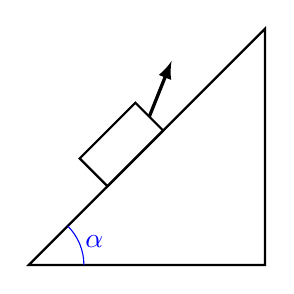
\begin{tikzpicture}[interface/.style={postaction={draw,decorate,decoration={border,angle=-45,amplitude=0.2cm,segment length=1.5mm}}},>=latex]
   \draw[thick] (0.5,0) -- (3.5,3) -- ++(0,-3) -- cycle;
   \draw[thick,rotate around={45:(1.5,1)}] (1.5,1) rectangle ++(1,0.5);
   \draw[very thick,rotate around={45:(1.5,1)},->] (2.5,1.25) --
   ++(0.7,0.3);
   \draw[blue] (1.2,0) arc (0:45:0.7) node[below=0.2cm,right=0.1cm] {$\alpha$};
\end{tikzpicture}
}

\taskpic{Тело массы $m_1$ лежит на доске массы $m_2$, находящейся на гладкой
  горизонтальной поверхности. Коэффициент трения между телом и доской
  $k$. Какую силу надо приложить к доске, чтобы тело соскользнуло с
  неё? За какое время тело соскользнёт, если к доске приложена сила
  $F_0$, а длина доски $l$?  }{
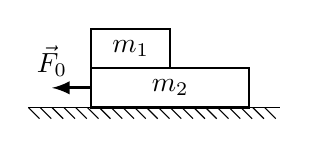
\begin{tikzpicture}[interface/.style={postaction={draw,decorate,decoration={border,angle=-45,amplitude=0.2cm,segment length=1.5mm}}},>=latex]
%  \draw[help lines,step=0.5] (0,0) grid (4,4);
  \draw[interface] (0.2,0) -- ++(3.2,0);
  \draw[thick] (1,0) rectangle ++(2,0.5) node[midway] {$m_2$};
  \draw[thick] (1,0.5) rectangle ++(1,0.5) node[midway] {$m_1$};
  \draw[very thick,->] (1,0.25) -- ++(-0.5,0) node[above] {$\vec{F}_0$};
\end{tikzpicture}
}

\taskpic{Между двумя одинаковыми гладкими брусками массами $m_1$ каждый
  вставлен клин массы $m_2$ с углом $\alpha$. Определите ускорение
  тел. }{
\begin{tikzpicture}[interface/.style={postaction={draw,decorate,decoration={border,angle=-45,amplitude=0.2cm,segment length=1.5mm}}}]
%  \draw[help lines,step=0.5] (0,0) grid (4,4);
  \draw[interface] (0.2,0) -- ++(3.6,0);
  \draw[thick] (0.5,0) rectangle ++(1,1.5) node[midway] {$m_1$}; 
  \draw[thick] (2.5,0) rectangle ++(1,1.5) node[midway] {$m_1$}; 
  \coordinate (a) at ($(1,2.25)!2!(1.5,1.5)$);
  \draw[thick] (1,2.25) -- (a) -- (3,2.25) -- cycle node[below=0.4cm,left=0.5cm]{$m_2$};
  \draw[blue] ($(a)!10pt!(3,2.25)$) arc (atan(3/2):90+atan(2/3):10pt)
  node[above=0.25cm,right=-0.05cm] {$\alpha$};
\end{tikzpicture}
}

%%% Local Variables: 
%%% mode: latex
%%% TeX-master: "../../../report"
%%% End: 
